\documentclass[12pt, letterpaper]{article}
\usepackage{graphicx}
\usepackage[
backend=biber,
style=alphabetic,
sorting=ynt
]{biblatex}
\usepackage{algpseudocode}
\usepackage{algorithm}
\usepackage{caption}
\usepackage{subcaption}
\usepackage{listings}
\addbibresource{bibliografie.bib}
\graphicspath{{images/}}
\title{Demonstrații zero-knowledge de apartenență la mulțimi}
\author{Andrei Pârjol}
\date{April 2024}

\begin{document}

\maketitle

\section{Introducere}

\subsection{Obiective} Obiectivul lucrării de față este acela de a prezenta și studia conceptele și implementările curente pentru protocoalele zk-SNARK folosite în demonstrațiile de apartenență la mulțimi. Deși pot părea abstracte la prima vedere , această ramură de demonstrații (in eng. \emph{zero-knowledge proof of membership}) are o gamă largă de aplicații precum : anonimizarea tranzacțiilor cu criptomonede (e.g. protocolul Zcash pentru Bitcoin și protocolul Tornado Cash pentru Ether), votul electronic descentralizat și anonim (e.g. putem să demonstrăm ca avem dreptul să votăm fără să dezvăluim date personale) sau mai general, folosirea anonimă a unor servicii online (e.g. fără să folosim username/password).

\subsection{Contribuția personală}

Pentru a arăta relevanța ideilor prezentate în această lucrare am scris o librărie JavaScript care implementeaza arborii hash Merkle și procedurile de generare și verificare a demonstrațiilor pentru apartenență folosind SNARK-uri. De asemenea se propun și îmbunătățiri , folosind arbori hash "\emph{indexați}" care reduc adancimea arborelui și implicit numărul de apeluri la funcția hash folosită in circuitul algebric.

\pagebreak

\section{Fundamente teoretice}
\subsection{Scurt istoric}
\vspace{5mm}
    Termenul de zero knowledge a fost propus prima dată la mijlocul anilor 1980 de către cercetătorii  Shafi Goldwasser , Silvio Micali și Charles Rackoff de la Institutul de tehnologie din Massachusetts . Ei încercau sa rezolve problemele legate de sistemele de demonstrare interactive , sisteme teoretice în care o parte numită Prover încearcă să convingă o altă parte numită Verifier că o propoziție matematică este adevărată.

    Acest tip de sistem este numit interactiv deoarece cele două părți interschimbă mesaje în timpul procesului de demonstrare și la vremea respectivă o mare parte din muncă era îndreptată înspre asigurarea validității sistemului, adică rezolvarea cazului în care Prover-ul avea intenții malițioase și încearca să păcălească Verifier-ul în a crede o propoziție falsă.

	În sistemele de demonstrare interactive este presupus că Demonstratorul are putere de calcul nelimitată (informal toate problemele sunt fezabile) însă nu este de încredere și Verificatorul are putere de calcul limitată și este onest. Ce au făcut cei trei cercetători a fost să ia în considerare și cazul în care Verificatorul nu este de încredere și s-au întrebat ce informații poate să obțină Verificatorul după o demonstrație. O astfel de scurgere de informații este destul de gravă deoarece din ipoteză folosind aceste sisteme Verificatorul are acces la informații pe care în mod normal nu ar fi putut să le calculeze. 

	A fost fost propusă astfel implementarea unui nou sistem , zero knowledge , în care se demonstrează cunoașterea unei soluții la o problemă în loc de soluție în sine . După terminarea demonstrației Verificatorul nu învață nimic nou în afara faptului că Demonstratorul cunoaște soluția.\cite{greenandblazewebsite}

 \subsection{Zero Knowledge}
 
 Dat fiind un sistem de demonstrație (P,V) și un Limbaj L (astfel încât $x\in L$ să fie echivalent cu x este adevărat ), acest sistem este zero knowledge dacă satisface următoarele trei proprietăți: 


\textbf{Completitudine} : $x\in L$  Pr[V acceptă ] = 1 . x este acceptat cu probabilitate 1 atunci când avem un demonstrator și verificator onest  .


\textbf{Corectitudine} : $x\in L$  Pr[V acceptă ] = 1/n , $n\in N$ . x este acceptat cu probabilitate redusă/mică  atunci când avem o demonstrație mincinosă și un verificator onest.


\textbf{Zero Knowledge} : Pentru orice verificator V exista o simulare S astfel încât orice rezultat final sau intermediar obținut de V se poate obține și de către S. Informal V nu poate să calculeze nimic din ce nu putea să calculeze înainte de verificarea demonstrației.

\subsection{zk SNARKs}
Este un obiect criptografic care poate să genereze într-un mod eficient un protocol zero knowledge pentru orice problemă sau funcție. 

zk SNARKs au următoarele proprietăți:
\begin{itemize}
\item {\textbf{zk} : intrările funcțiilor rămân ascunse} 
\item{\textbf{Succint} : demonstrațiile generate sunt scurte și pot fi verificate rapid.}
\item{\textbf{Noninteractive} : nu este necesară comunicarea prin întrebări și răspunsuri dintre Demonstrator și Verificator.}
\item{\textbf{ARgument of Knowledge} : se demonstrează cunoașterea unei intrări x pentru o funcție și un rezultat dat.}
\end{itemize}
Ideea de bază:
Se transformă problema (ex: logaritm discret , colorarea grafului etc.) într-o funcție a cărei intrări vrem să le ascundem.
Executăm funcția folosind criptarea homeomorfă și funcția este apoi trecută printr-un procedeu numit “roll up” în care se obține o semnătură scurtă care indică execuția corectă a funcției.

\pagebreak
\section{Acumulatori criptografici}
Un acumulator criptografic este o reprezentare compactă a unei mulțimi de elemente sub forma unui hash. 

Această reprezentare permite generarea de demonstrații de apartenență scurte, notate $w_x$ și numite witness(martor),pentru orice element $x$ care a fost acumulat sau demonstrații de non-apartenență pentru orice element din domeniu care nu a fost acumulat.

Acumulatorii care suportă doar demonstrații de apartenență sunt numiți \emph{pozitivi}, cei care suportă doar demonstrații de non-apartenență sunt numiți \emph{negativi} iar cei care suportă ambele tipuri de demonstrații sunt numiți \emph{universali}.

O altă clasificare pentru acumulatori este dată de metodele de actualizare pe care aceștia le suportă, astfel avem acumulatori:
\begin{itemize}
    \item{\textbf{aditivi} - suportă doar introducerea de elemente noi în mulțime}
    \item{\textbf{substractivi} - suportă doar eliminarea de elemente din mulțime}
    \item{\textbf{dinamici} - suportă ambele operații descrise mai sus}
\end{itemize}

Dacă avem o entitate(trusted party) responsabilă pentru actualizarea acumulatorului acesta se numește \emph{trapdoor-based} altfel acesta se numește \emph{trapdoorless}.

Pentru acumulatorii \emph{trapdoor-based}, entitatea responsabilă pentru actualizarea mulțimii suport se numește \emph{managerul acumulatorului}. Acesta deține o cheie secretă (\emph{trapdoor}) și este capabil să adauge , să șteargă elemente și să genereze demonstrații într-un mod eficient.

Acumulatorii \emph{trapdoorless} permit actualizări publice asupra mulțimii suport, fără a mai fi nevoie de o parte terță de încredere. Astfel utilizatorii sunt responsabili pentru actualizarea și generarea de demonstrații.


Acumulatorii criptografici au numeroase aplicații,cele mai populare fiind : anonymous credentials , group signatures, stocarea datelor in cloud și anonimizarea tranzacțiilor cu criptomonede.
\cite{cryptoeprint:2023/1001}

\subsection{Date private și scalabilitate}

Din definiția dată mai sus acumulatorii criptografici nu au nicio propietate care să păstreze datele private. O parte malițiosă poate să afle pentru ce element din mulțime s-a făcut o demonstrație sau poate să afle ce element a fost șters sau adăugat în acumulator. Aceste informații pot fi folosite pentru a falsifica demonstrații și pentru a actualiza abuziv mulțimea/acumulatorul.

În practică acumulatorii sunt folosiți în zone în care datele trebuie să rămână private așa că demonstrațiile convenționale sunt înlocuite cu demonstrațiile \emph{zero-knowledge}. Odată cu schimbarea tipului de demonstrație folosit apar și probleme noi pe care le vom discuta și rezolva în continuare : \emph{replay attacks} - folosirea repetată a aceleiași demonstrații, timpi de lucru mari pentru generarea demonstrațiilor și probleme de concurență atunci cand doi sau mai mulți utilizatori încearcă să actualizeze același acumulator în același timp.

Dorim totodată ca acumulatorul să fie scalabil și să ne permită să verificăm apartenența $x \in S$ într-un timp subliniar, fără să reținem toate elementele din $S$.

Pentru a realiza cele două obiective trebuie să definim părțile care participă în procesul de demonstrare : 
\begin{itemize}
    \item{\textbf{Prover} - cunoaște valoarea secretă $x$ și mulțimea $S$ și are spațiu de memorie și putere de calcul nelimitate. Acesta este responsabil de generarea demonstrației de apartenență.}
    \item{\textbf{Verifier} - nu cunoaște valoarea secretă $x$ sau mulțimea $S$ și deține spațiu de memorie și putere de calcul limitate. Acesta este responsabil de verificarea demonstrației de apartenență.  }
\end{itemize}

Împărțind problema celor două roluri putem să păstrăm datele private și să obținem scalabilitate.

\subsection{Verificarea eficientă a demonstrațiilor}

Formal un acumulator poate fi descris printr-un triplet de 3 algoritmi : $(Acc,Prove,Verify)$ care au următoarele funcționalități:
\begin{itemize}
    \item{\textbf{$A \leftarrow Acc(S)$} - realizează compresia mulțimii $S$ într-o valoare scurtă notată cu A.}
    \item{\textbf{ $\pi_x \leftarrow Prove(x,S)$} - generează demonstrația de apartenență la mulțimea $S$ pentru elementul $x$.}
    \item{\textbf{ $\{0,1\} \leftarrow Verify(A,x,\pi_x)$} - acceptă sau respinge demonstrația $\pi_x$ folosind doar valoarea comprimată $A$.}
\end{itemize}

Pentru a fi considerate eficiente, dimensiunea acumulatorului $A$ , a demon-
strației $\pi_x$ și complexitatea timp a algoritmului $Verify$ trebuie să fie mai mici decât $|S|$. În continuare sunt prezentați arborii hash Merkle în care algoritmul $Verify$ are o complexitate timp $O(log(|S|))$. 

\subsection{Arbori hash Merkle - $Acc(S)$}
Arborii hash Merkle sunt arbori binari în care valoarea fiecărui nod este dată de o funcție hash criptografică care primește ca și intrări valorile copiilor nodului, sau dacă nodul este nod frunză primește cheile secrete din mulțimea suport. 

Funcția hash folosită intr-un arbore Merkle este importantă deoarece în contextul zero-knowledge dorim o funcție care sa fie ușor de scris sub-forma unui circuit algebric pentru a genera un SNARK cât mai eficient și cu cât mai puține constrângeri. Astfel de funcții hash sunt numite și \emph{"zk-friendly"}, iar câteva funcții folosite în practică sunt  : Poseidon \cite{cryptoeprint:2019/458} , MiMC \cite{cryptoeprint:2016/492} , Vision Mark-32 \cite{cryptoeprint:2024/633} sau Rescue \cite{cryptoeprint:2022/1577}. În implementarea prezentată în această lucrare vom folosi funcția hash Poseidon , prescurtată cu POS.

În Figura \ref{fig:arbore_hash1} de mai jos este prezentat un arbore hash de adâncime 3 în care am acumulat cheile secrete $S=\{A,B, \dots ,F\}$. Nodurile frunză conțin doar hash-urile $\{POS(A),POS(B), \dots ,POS(F)\}$, iar nodurile care nu au o valoare setată primesc o valoare \emph{null} notată cu \emph{zeroVal} sau \emph{0}. 

Folosirea unei valori \emph{null} prestabilită ne permite să implementăm într-un mod eficient arbori Merkle \emph{sparse} care au o adancime foarte mare însă puține elemente deoarece putem să calculăm valorile null pentru fiecare nivel de adâncime.

Arborii Merkle au o proprietate adițională care îi face mai puternici decât alți acumulatori criptografici deoarece realizează un \emph{"vector commitment"} : rădăcina arborelui codifică nu numai conținutul mulțimii dar și ordinea în care elementele apar în mulțime/vector și astfel este imposibil pentru un Prover să demonstreze două valori diferite la aceiași poziție. 

\pagebreak
\begin{figure}[h]
\centering
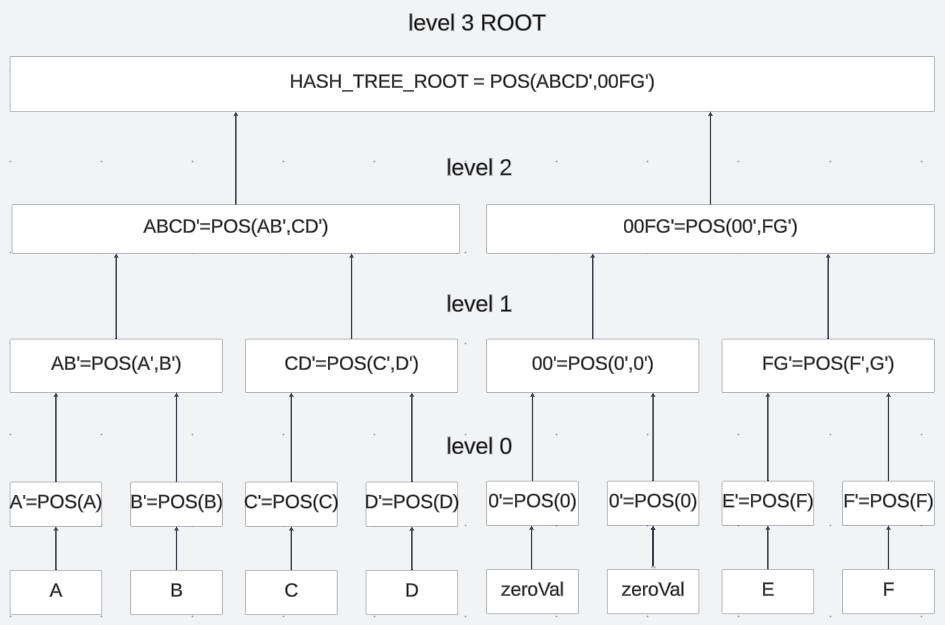
\includegraphics[width=1\textwidth]{hashtree.png}
\caption{Arbore Merkle sparse de adâncime 3 }
\label{fig:arbore_hash1}
\end{figure}

\subsection{Demonstrații de apartenență - $Prove(x,S)$}

O demonstrație de apartenență în contextul arborilor Merkle presupune  parcurgerea corectă a drumului de la nodul frunză cu valorea $POS(x)$ pentru care se face demonstrația până la rădăcina arborelui.

Funcția $Prove(x,S)$ generează vectorii de lungime $\lfloor log(|S|) \rfloor$ : \emph{siblings} - vectorul cu fiecare nod frate din fiecare nivel și \emph{path} - vectorul care codifică poziția nodului curent în funcția hash pentru a calcula nodul următor. În implementare folosim 0 pentru stânga și 1 pentru dreapta. Pe lângă cei doi vectori care atestă că elementul face parte din mulțimea $S$ la poziția indicată , un Prover mai trebuie să demonstreze și faptul că știe preimaginea valorii $POS(x)$ prin funcția hash aleasă , printr-o semnatură a unui mesaj sau un circuit zk-SNARK simplu.

În Figura \ref{fig:demonstrație_arbore_hash} de mai jos sunt colorate cu verde toate nodurile care fac parte din vectorul $siblings_C$ pentru demonstrația de apartenență a elementului $C$.

\pagebreak

\begin{figure}[ht]
    \centering
    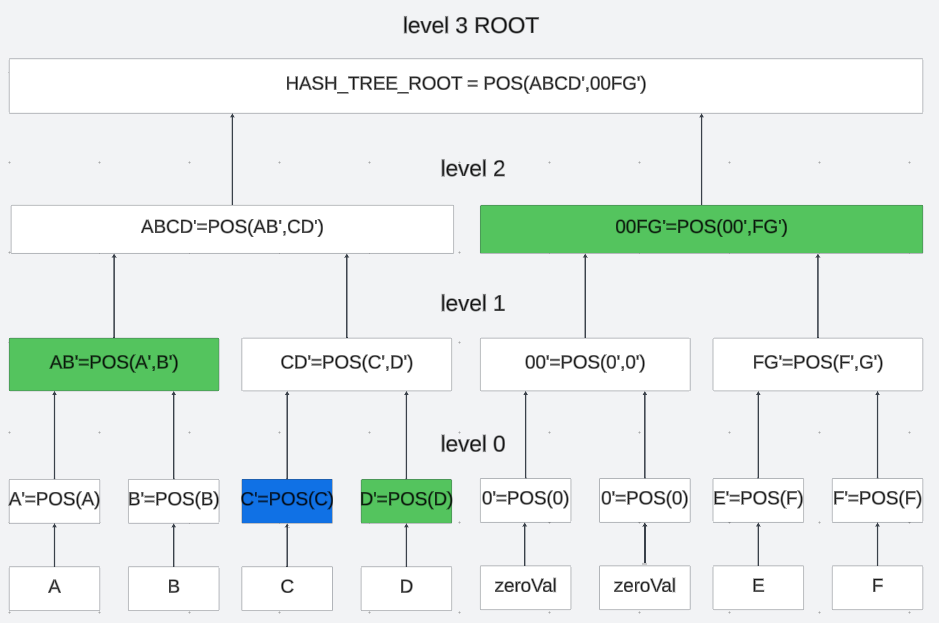
\includegraphics[width=1\textwidth]{hashtreeProof.png}
    \caption{Demonstrație pentru nodul cu cheia secretă $C$}
    \label{fig:demonstrație_arbore_hash}
\end{figure}

În acest exemplu , $Prove(x,S)$ generează vectorii $siblings_C= [ D',AB',00FG' ],$
$path_C=[0,1,0]$ împreună cu preimaginea C sau o semnatură/demonsrație zk pentru cheia secretă C.

\subsection{Verificarea demonstrației - $Verify(A,x,\pi_x)$}

Verificarea unei demonstrații Merkle presupune verificarea semnături și recalcularea rădăcinii arborelui folosind vectorii $siblings$ și $path$ și funcția publică hash.

Dacă rădăcinia calculată este egală cu rădăcina arborelui Merkle atunci demonstrația este acceptată altfel este respinsă.

Verifier-ul poate să evalueze o astfel de demonstrație într-un timp logaritmic și fără să salveze în memorie întreg arborele. Deși eficientă, acestă metodă de demonstrare nu păstrează datele private deoarece Verifier-ul află semnatura și poziția hash-ului cheii secrete în arbore.

\section{Demonstrații de non-apartenență}
Potrivit definiției de mai sus un arbore hash Merkle este un acumulator criptografic \emph{dinamic}, care suportă operațiile de inserare,actualizare și ștergere, însă în practică nu dorim să executăm operațiile de actualizare sau ștergere deoarece acestea pot duce la scurgeri de informații cu privire la nodurile care au fost actualizate.

\subsection{Modelul UTXO}
Pentru a elimina un nod dintr-un arbore Merkle acesta trebuie \emph{anulat} folosind un \emph{nullifier}. Un nullifier este un hash-commitment compus din cheia secretă a nodului si ID-ul arborelui Merkle din care face parte , prin care se indică faptul că nodul a fost "consumat".În cazul in care dorim să actualizăm valoarea unui nod , trebuie sa anulăm nodul vechi și sa inserăm un nod cu valoarea nouă. 

Valoarea unui nullifier , de obicei un hash , nu trebuie să dezvăluie ce nod anulează din arborele hash și este de obicei salvată într-un alt arbore Merkle sparse numit \emph{"Nullifier tree"}. Acest model cu doi arbori hash se numește UTXO Model (eng. \emph{Unspent Transactions Outputs}) și este folosit de exemplu în gestionarea tranzacțiilor cu criptomonede. Modelul UTXO este util deoarece rezolvă o problemă de securitate în ceea ce privește demonstrațiile uzuale: replay attacks - folosirea repetată a aceleiași demonstrații.\cite{stanford_blockchain:2022}

Pentru a demonstra apartenența unui element $x$ în modelul UTXO trebuie să demonstrăm că $POS(x)$ face parte din arborele hash și faptul ca nullifier-ul asociat cheii secrete nu se află in nullifier Tree. 

\begin{figure}[ht]
    \centering
    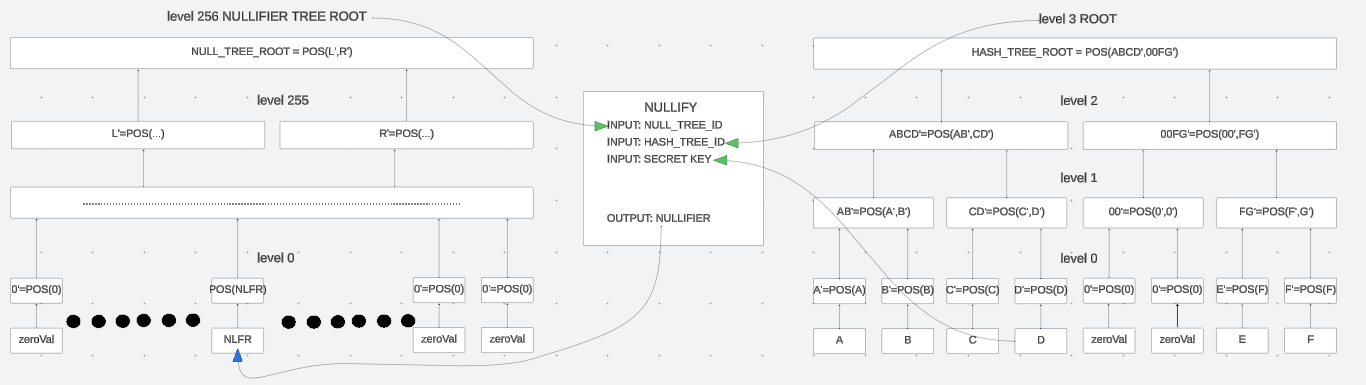
\includegraphics[width=1\textwidth]{images/nullify.png}
    \caption{Calculul unui nullifier pentru elementul cu cheia secretă "D"}
    \label{fig:nullify_calc}
\end{figure}

\subsection{Verificarea în modelul UTXO }
Arborele nullifier \emph{nullTree} este un arbore hash sparse cu suficiente noduri frunză pentru a cuprinde toate valorile posibile pentru funcția hash folosită. În cazul nostru , funcția hash \emph{POSEIDON} generează valori în câmpul prim $Z_p$ , p fiind numărul de elemente (ordinul) câmpului generat de curba eliptică ALT\_BN128 \cite{eip196}. Numărul p se află între $2^{253}\leq p\leq 2^{254}$ , așa că avem nevoie de un arbore hash cu 254 de nivele pentru a putea acomoda toate valorile din domeniul funcției $POS$.

Putem să folosim valorile hash / nullifier pe post de index în vectorul nodurilor frunză și să codificăm valorile 0 pentru nefolosit și 1 pentru folosit.

Demonstrația de non-aparteneță pentru un anumit nullifier/valoare hash revine la o demonstrație de apartenența a elementului "0" la poziția nullifier-ului. În acest mod putem verifica în timp constant \emph{$O(1)$} dacă un nullifier a fost folosit sau nu. 

Structura sparse a arborilor hash ne permite o verificare ușoară a non apartenenței iar demonstrația nu dezvăluie informații noi pentru Verifier deoarece funcția care leagă un nullifier de cheia pe care o anulează este o funcție hash criptografică.

Demonstrația zero knowledge completă va trebui să conțină următoarele:
\begin{itemize}
    \item{demonstrația de apartenență în arborele hash pentru cheia secretă}
    \item{demonstrația că nullifier-ul a fost calculat corect}
    \item{demonstrația de non-apartenență în arborele nullTree pentru nullifier}
\end{itemize}

\subsection{Problemele arborilor hash sparse}

Desi demonstrația de non-apartență este simplă și are un timp constant aceasta nu poate să fie folosită în mod eficient în SNARK-uri deoarece arborele are o adâncime foarte mare și necesită executarea funcției hash pentru fiecare nivel. Funcțiile hash reprezintă o operație foarte costisitoare în contextul circuitelor algebrice folosite în SNARK-uri și deși există funcții hash optimizate pentru acest mediu, expuse mai sus, faptul ca trebuie să apelăm funcția hash de 254-ori pentru a demonstra non-apartenența unui nullifier va duce la probleme de scalabilitate.


\section{Arbori hash indexați}
O soluție pentru această problemă de performanță este prezentată în \cite{cryptoeprint:2021/1263} unde se propune idea de \emph{arbore Merkle indexat}, un arbore care ne permite să facem demonstrații zero-knowledge de non-apartenență eficiente.

Acest arbore este dens, are o adâncime substanțial mai mică și nodurile frunză reprezintă \emph{hash commitment}-urile nodurilor unui lanț circular simplu înlânțuit de hash-uri nullifier ordonate în ordine crescătoare.

Structura nodului din lanț este compusă din: valoarea nullifier-ului $nlfr\in F_p$, valoarea nullifier-ului următor in ordine crescătoare $nlfr_{next}$ și index-ul următorului nullifier $i_{next}$.

\centering

$leafnode = \{nlfr, i_{next}, nlfr_{next}\}$

\raggedright

În arborele nullTree sunt introduse doar hash commitment-urile calculate folosind funcția POSEIDON , POS([$nlfr, i_{next}, nlfr_{next}$]).

Regula de inserție pentru un nullifier nou este aceiași cu cea pentru un lanț simplu înlănțuit normal , în care schimbăm pointerii pentru a păstra ordinea crescătoare a valorilor hash. 

Această regulă de inserție și structura ordonată a lanțului generează o propeitate importnată pe care o vom folosi mai departe : dacă un nod de forma $leafnode = \{nlfr, i_{next}, nlfr_{next}\}$ face parte din lanț atunci nu există niciun nullifier care a fost deja folosit în intervalul $(nlfr,nlfr_{next})$ .
Cu această proprietate putem să demonstrăm foarte simplu dacă un nullifier face sau nu parte dintr-un arbore indexat.

\subsection{Construcția arborelui și algoritmul de inserție}

Construcția arborelui indexat presupune un nivel adițional folosind un vector, în care vom păstra lanțul simplu înlănțuit compus din obiecte cu 3 proprietăți: valoarea hash-ului ,index-ului hash-ului următor și valoarea hash-ului următor.

Inițial arborele conține valorile $HASH\_MIN=0\ și\ HASH\_MAX=p-1$ (unde p-1 este valoarea "maximă" din câmpul $F_p$) și lanțul este compus din $LINKED\_LIST=[\{0,1,p-1\},\{p-1,0,0\}]$ . Riscul de coliziune cu un alt nullifier este neglijabil iar aceste 2 margini, inferioare și superioare, ne reduc câteva cazuri speciale din algoritmul de inserție. 

Algoritmul implică căutarea unui nod cu valoarea hash-ului mai mică decât hash-ul inserat $nlfr < new\_hash$ și valoarea hash-ului următor mai mare decât hash-ul inserat $new\_hash < nlfr_{next}$.

\begin{algorithm}
    \caption{Algoritm pentru inserarea hash-urilor într-un arborele indexat}
    \label{index_tree_hash_insert_alg}
    \begin{algorithmic}[1]
        \Function{insertHashValue}{$nullTree,hashValue$}
            \State $current\_node \gets nullTree.LinkedList[0]$
            \State $next\_index \gets current\_node.next\_index$ 
            \While{$next\_index\not=0$}\Comment{cât timp nu am parcurs toată lista}
                \State $current\_hash \gets current\_node.hash\_value$
                \State $next\_hash \gets current\_node.next\_hash\_value$
                \If { ($current\_hash<hashValue)\ \&\&\ (hashValue<next\_hash$) } 
                  \State \textbf{break}
                \Else 
                \State $current\_node\gets nullTree.LinkedList[next\_index]$
                \State $next\_index \gets current\_node.next\_index$ 
                \EndIf
            \EndWhile
            \If {$next\_index=0$}
                \State \textbf{throw new Error("Hash already inserted!")}
            \Else 
                \State $new\_node = new\ LeafNode()$
                \State $new\_node.hash\_value\gets hashValue$
                \State $new\_node.next\_index\gets next\_index$
                \State $new\_node.next\_hash\_value\gets current\_node.next\_hash\_value$
                \State $nullTree.LinkedList.push(new\_node)$
                \State $current\_node.next\_index\gets nullTree.LinkedList.length-1$
                \State $current\_node.next\_hash\_value\gets new\_node.hash\_value$      
            \EndIf
        \EndFunction
    \end{algorithmic}
\end{algorithm}

Algoritmul inserează valoarea $hashValue$ în arborele indexat $nullTree$ dacă aceasta nu există în arbore altfel aruncă o eroare deoarece hash-ul a fost deja inserat.

În exemplul următor este prezentat un arbore indexat de adâncime 3 (8 noduri frunză) în care inserăm în ordine valorile hash $\in F_p$ : $10,20,15,5$. Fiecare schimbare este evidențiată cu culoarea verde-deschis.

\begin{figure}[ht]
    \centering
    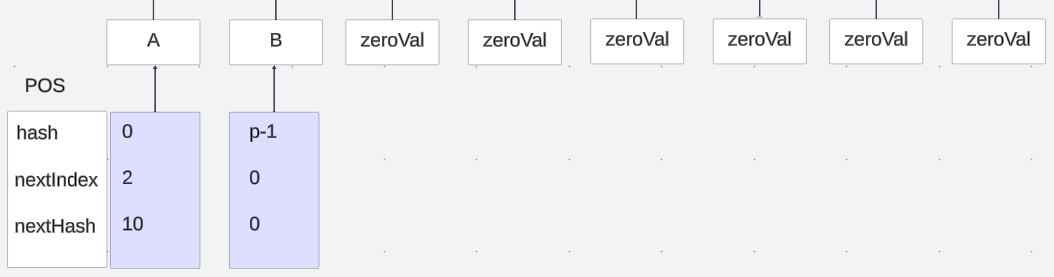
\includegraphics[width=1\textwidth]{images/nullTreeInsert/nullTreeInsertInitial.png}
    \label{fig:nullTreeInsertInitial}
\end{figure}

\begin{figure}[ht]
    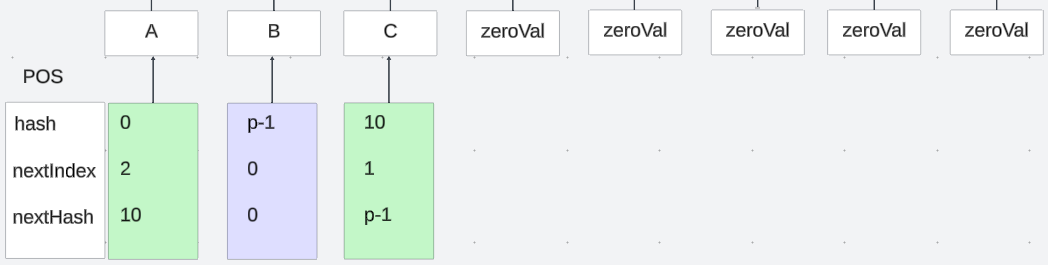
\includegraphics[width=1\textwidth]{images/nullTreeInsert/nullTreeInsert10.png}
    \label{fig:nullTreeInsert10}
\end{figure}

\begin{figure}[ht]
    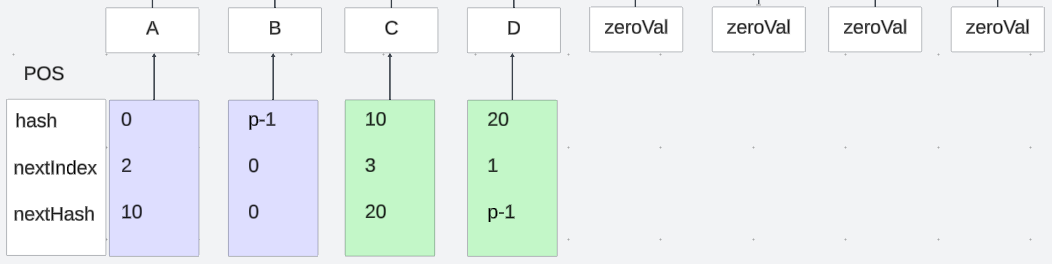
\includegraphics[width=1\textwidth]{images/nullTreeInsert/nullTreeInsert20.png}
    \label{fig:nullTreeInsert20}
\end{figure}

\begin{figure}[ht]
    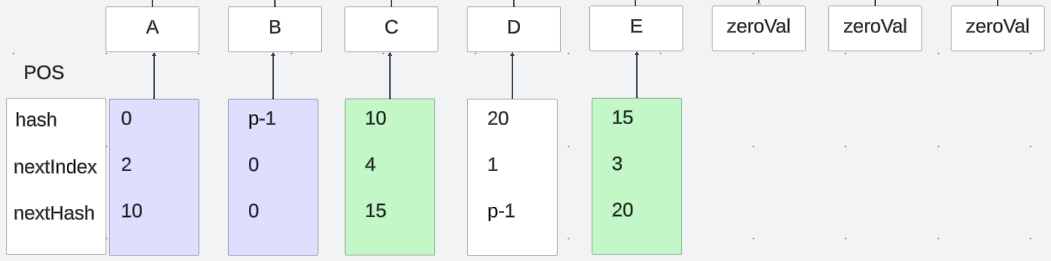
\includegraphics[width=1\textwidth]{images/nullTreeInsert/nullTreeInsert15.png}
    \label{fig:nullTreeInsert15}
\end{figure}

\begin{figure}[ht]
    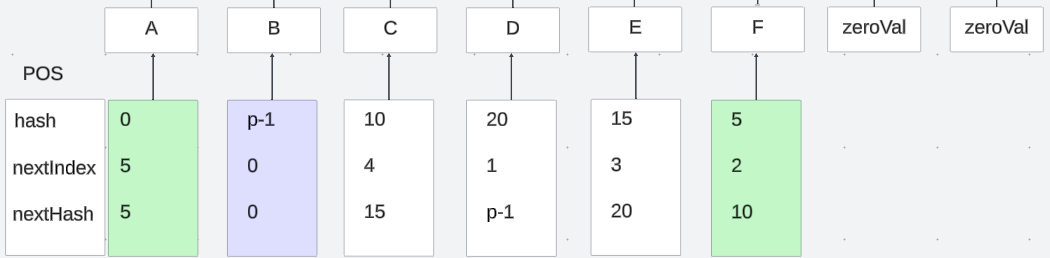
\includegraphics[width=1\textwidth]{images/nullTreeInsert/nullTreeInsert5.png}
    \label{fig:nullTreeInsert5}
\end{figure}

\newpage

După ce a fost inserat un nod nou trebuie să recalculăm hash commitment-ul atât pentru nodul nou cât și pentru nodul actualizat, adică cele două noduri colorate cu verde din exemplul precedent și apoi să recalculăm rădăcina arborelui indexat.

\section{Implementarea protocolului folosind Circom 2.0 și snarkJS}

În această secțiune sunt prezentate limbajul Circom , biblioteca snarkJS și implementările tuturor circuitelor folosite în protocolul de demonstrare a apartenenței folosind arbori indexați și arbori hash.

\subsection{Circom 2.0}

Circom este un limbaj low-level și un compilator pentru circuite scris în Rust. Acesta este folosit împreună cu librăria snarkJS pentru a genera și testa demonstrații zero-knowledge eficiente.

Limbajul lucrează cu un singur tip de date, numit semnal(eng. signal) care poate avea diverse nivele de acces : public/privat și care pot fi folosite în diverse părți ale unui circuit : semnale de intrare , semnale intermediare și semnale de ieșire. Dacă nu este specificat altfel semnalele de intrare sunt private. Semnalele intermediare sunt private și nu pot fi modificate iar semnalele de iesire sunt publice și nu pot fi modificate. Semnalele pot lua valori doar din câmpul finit $F_p$ unde p este ordinul câmpului generat de curba eliptică ALT\_BN128.\cite{eip196}

Fiecare circuit împreună cu semnalele sale trebuie să aibe forma unui QAP, Quadratic Arithmetic Program, adică fiecare semnal intermediar sau de ieșire are forma : 

$signalOUT === (A*signalINTER1+B)*(C*signalINTER2+D)$
unde $A,B,C,D \in F_P$.

Pe lângă operatorii aritmetici clasici , Circom folosește și operatori care vor fi folosiți la compilare pentru generarea de constrângeri asupra semnalelor. Avem astel operatorul de constrângere "===" , operatorul de atribuire fără constrângere (la stânga/dreapta) $<--$/$-->$ și operatorul de atribuire împreună cu constrângere (la stânga/dreapta) $<==$/$==>$


Scrierea circuitelor , notate cu \emph{Template} atunci când sunt definite și cu \emph{Component} atunci când sunt instanțiate, permite o dezvoltare modulară deoarece semnalele de ieșire ale unui circuit pot fi redirecționate către semnalele de intrare ale unui alt circuit.

Odată scrise circuitele pot fi construite și compilate în fișiere *.r1cs, formatul sistemelor de constrângeri, Rank 1 Constraint System.

\subsection{snarkJS}

snarkJS este o bibliotecă JavaScript care face parte din ecosistemul circom. Este responsabilă de generarea \emph{trusted setup}-ului și a cheilor de verificare și demonstrare pentru diverse protocoale snark precum : GROTH16, PLONK și FFLONK.

Folosind funcțiile din biblioteca snarkJS putem să generăm și să verificăm demonstrații zero-knowledge în browser/server sau într-un mediu decentralizat precum Ethereum EVM folosind contractele solidity generate de către circom.

\pagebreak
\subsection{Circuite utilitare}

Circuitele utilitare prezentate mai jos nu au legătură directă cu protocolul de demonstrare a apartenenței însă aduc un nivel ridicat de modularitate și separă funcționalitatea codului.Acestea rezolvă o problemă care apare în Circom atunci când incercăm să comparăm valori foarte mari(apropiate de numărul p, ordinul câmpului ).

Un dezavantaj al limbajului Circom este faptul că semnalele pot lua valori doar în câmpul $F_p$ și nu pot avea valorile \emph{true/false} deci nu putem folosi operatorii de comparație ($<,>,=,\leq$) cu operanzi semnale. 

Libraria standard Circom implementează doua circuite \emph{"LessThan" și "GreaterThan"} însă acestea sunt limitate la valori $\leq2^{252}$,deoarece operațiile de comparație nu sunt atât de comune, și nu acopera toate valorile posibile din domeniul funcției hash POSEIDON, valori hash pe care dorim să le comparăm.

Pentru a putea compara toate valorile vom transforma întâi fiecare număr în reprezentarea sa binară pe 256 biți(reprezentarea cu cel mai important bit la dreapta) , vom segmenta apoi fiecare secvență binară în 4 părți de 64 biți pe care le vom converti înapoi în elemente din $F_p$ și pe care le comparăm cu circuitul "LessThan" din librăria standard. Reducem astfel cele 2 numere la 2 secvențe de 4 biți pe care le convertim la elemente din $F_p$ și le comparăm încă o dată pentru a determina rezultatul final. 

\begin{lstlisting}[caption="Num2Bits.circom"]
template Num2Bits(n){
    signal input in;
    signal output out[n];

    var value = 0;
    var pow = 1;
    for(var i=0;i<n;i++){
        out[i] <-- (in>>i)&1;
        out[i]*(1-out[i]) === 0;
        value += out[i]*pow;
        pow += pow;
    }

    value === in;}
\end{lstlisting}

Circuitul \textbf{Num2Bits(n)} este folosit pentru a genera secvența binară  de lungime $n$ asociată numarului trimis prin semnalul de intrare \textbf{in}. Avem $n$ semnale de ieșire corespunzatoare fiecărui bit , cel mai important fiind pe poziția \textbf{out[255]} (Most significant bit right). În implementare vom folosi $n=256$.

\begin{lstlisting}[caption="Bits2Num.circom"]
template Bits2Num(n){
    signal input in[n];
    signal output out;

    var value = 0;
    var pow = 1;
    for(var i=0;i<n;i++){
        in[i]*(1-in[i]) === 0;
        value += pow*in[i];
        pow +=pow;
    }
    out <== value;
}
\end{lstlisting}

\textbf{Bits2Num(n)} este folosit pentru a calcula elementul din $F_p$ echivalent cu secvența binară trimisă prin cele $n$ semnalele de intrare \textbf{in[n]}.
Rezultatul este calculat modulo $p$ și trimis prin semnalul de ieșire \textbf{out}.

\begin{lstlisting}[caption="LessThan"]
template LessThan(){
    signal input in[2];
    signal output out;

    component n2b = Num2Bits(253);

    n2b.in <== in[0]+(1<<252)-in[1];
    out <== 1-n2b.out[252];
}
\end{lstlisting}

Circuitul \textbf{LessThan} face parte din librăria standard Circom. Acesta primește 2 semnale de intrare \textbf{in[0]} și \textbf{in[1]} și returnează prin semnalul de ieșire \textbf{out} : 1 dacă $in[0]<in[1]$ și 0 altfel.

\begin{lstlisting}[caption="isZero.circom"]
template isZero(){
    signal input in;
    signal output out;

    signal inv <-- in == 0 ? 0 : 1/in;
    out <== 1 - in*inv;
    out*in === 0;
}
\end{lstlisting}
\textbf{isZero} face parte din librăria standard Circom. Acesta primește un singrul semnal de intrare \textbf{in} și returnează prin semnalul de ieșire \textbf{out} : 1 dacă semnalul de intrare este 0 și 0 altfel.

\begin{lstlisting}[caption="isEqual.circom"]
include "./isZero.circom";

template isEqual(){
    signal input in[2];
    signal output out;
    component checkZero = isZero();
    checkZero.in<== in[0]-in[1];
    out<==checkZero.out;
}
\end{lstlisting}
Circuitul \textbf{isEqual} face parte din librăria standard Circom. Acesta primește două semnale de intrare \textbf{in[0]} și \textbf{in[1]} , calculează diferența dintre cele două pe care apoi o trimite ca și semnal de intrare  într-un circuit "isZero". Semnalul de ieșire este preluat de la semnalul de ieșire al circuitului isZero folosit.

\pagebreak
\subsection{Circuitul LessThan\_256BIT\_MSBR}

\begin{lstlisting}[caption="LessThan\_256BIT\_MSBR"]
include "./Num2Bits.circom";
include "./Bits2Num.circom";
include "./LessThan.circom";
include "./isEqual.circom";

template LessThan_256BIT_MSBR(){
    signal input in[2];
    signal inter1[4];
    signal inter2[4];
    signal output out;
    component n2b = Num2Bits(256);
    component b2n[4] ;
    n2b.in <== in[0];
    for(var i=0;i<4;i++){
        b2n[i] = Bits2Num(64);
        for(var j=0;j<64;j++){
            b2n[i].in[j]<==n2b.out[j+(64*i)];
        }
        inter1[i]<==b2n[i].out;
    }
    component n2b_2 = Num2Bits(256);
    component b2n_2[4] ;
    n2b_2.in <== in[1];
    for(var i=0;i<4;i++){
        b2n_2[i] = Bits2Num(64);
        for(var j=0;j<64;j++){
            b2n_2[i].in[j]<==n2b_2.out[j+(64*i)];
        }
        inter2[i]<==b2n_2[i].out;
    }

    signal interBINcomp1[4];
    signal interBINcomp2[4];
    component interLT[4];
    component isEq[4];

    for(var i=0;i<4;i++){
        interLT[i] = LessThan();
        isEq[i] = isEqual();
        interLT[i].in[0]<==inter2[i];
        interLT[i].in[1]<==inter1[i];
        isEq[i].in[0]<==inter2[i];
        isEq[i].in[1]<==inter1[i];
        interBINcomp1[i]<== interLT[i].out;
        interBINcomp2[i]<== (1-interLT[i].out)-isEq[i].out;
    }

    signal num[2];
    component b2n_f[2];
    b2n_f[0]=Bits2Num(4);
    b2n_f[0].in[0]<== interBINcomp1[0];
    b2n_f[0].in[1]<== interBINcomp1[1];
    b2n_f[0].in[2]<== interBINcomp1[2];
    b2n_f[0].in[3]<== interBINcomp1[3];
    b2n_f[1]=Bits2Num(4);
    b2n_f[1].in[0]<== interBINcomp2[0];
    b2n_f[1].in[1]<== interBINcomp2[1];
    b2n_f[1].in[2]<== interBINcomp2[2];
    b2n_f[1].in[3]<== interBINcomp2[3];

    num[0]<== b2n_f[0].out;
    num[1]<== b2n_f[1].out;

    component LTF = LessThan();
    LTF.in[0]<==num[0];
    LTF.in[1]<==num[1];
    out<==LTF.out;
}
\end{lstlisting}
Circuitul \textbf{LessThan\_256BIT\_MSBR} folosește toate cele 5 circuite prezentate mai sus și extinde circuitul \emph{LessThan} deoarece permite compararea tuturor valorilor din $F_p$. Pentru a trece de limitarea circuitului \emph{LessThan} din librăria standard, vom reprezenta valorile semnalelor de intrare \textbf{in[0]} și \textbf{in[1]} pe 256 biți și vom compara pe rând 4 segmente de 64 biți din fiecare secvență. Dacă un segment este mai mare atunci îl înlocuim cu 1, altfel îl înlocuim cu 0. La sfârșit semnalele de intrare ajung să conțină 2 secvențe de 4 biți , care sunt convertite inapoi la elemente din $F_p$ folosind circuitul \emph{Bits2Num} și comparate cu \emph{LessThan} pentru a returna rezultatul final: 1 dacă $in[0]<in[1]$ și 0 altfel.

\subsection{Circuite secundare}
În acestă secțiune sunt prezentate circuitele secundare create pentru a realiza demonstrații în arbori hash normali și indexați.

\begin{lstlisting}[caption="Selector.circom"]
template Selector(){
    signal input switcher;
    signal input in[2];
    signal int[4];
    signal output out[2];
    0 === (switcher)*(1-switcher);
    int[0] <== in[0]*(1-switcher);
    int[1] <== in[1]*switcher;
    out[0] <== int[0] + int[1];

    int[2] <== in[1]*(1-switcher);
    int[3] <== in[0]*switcher;
    out[1] <== int[2] + int[3];

}
\end{lstlisting}

\textbf{Selector} este folosit pentru a seta semnalele de intrare ale funcției hash POSEIDON pentru fiecare nivel din arbore. Circuitul primește 3 semnale de intrare , \textbf{in[0], in[1] și switcher}, și returnează semnalele inversate dacă $switcher=1$ , altfel returnează aceleași semnale. În generarea demonstrațiilor, pentru fiecare vector de hash-uri \emph{"siblings"} este generat și un vector de aceiași dimensiune,numit \emph{path}, ce conține codificările poziției (0-stânga și 1-dreapta) hash-ului curent pentru a calcula următorul hash. Circuitul este apelat întotdeauna cu hash-ul curent prin \textbf{in[0]} și cu hash-ul sibling prin \textbf{in[1]}.


\begin{lstlisting}[caption="HashTreeLevel.circom"]
include "../node_modules/circomlib/circuits/poseidon.circom";
include "./Selector.circom";

template HashTreeLevel(){
    signal input in[2];
    signal input position;
    signal output out;

    component poseidon = Poseidon(2);
    component selector = Selector();

    selector.in[0] <== in[0];
    selector.in[1] <== in[1];
    selector.switcher <== position;

    selector.out[0] ==> poseidon.inputs[0];
    selector.out[1] ==> poseidon.inputs[1];

    poseidon.out ==> out;

}
\end{lstlisting}
\textbf{HashTreeLevel} este folosit pentru a calcula următorul nivel dintr-un arbore Merkle dat. Circuitul primește hash-ul din nivelul anterior împreună cu hash-ul sibling din nivelul curent și ordinea în care apar în apelul funcției hash POSEIDON. Acest ciruit este folosit exclusiv în demonstrațiile de apartenență în arbori hash simpli, în timp ce demonstrațile de apartență în arbori indexați au o structură similară dar necesită mai multe verificări și constrângeri și sunt tratate direct în circuitul principal.
\pagebreak

\subsection{Circuitul principal}
\begin{lstlisting}[caption="MainProof.circom"]
include "../node_modules/circomlib/circuits/poseidon.circom";
include "./HashTreeLevel.circom";
include "./LessThan_256BIT_MSBR.circom";

template MainProof(depth){
    signal input sk;
    signal input siblingsPk[depth];
    signal input path[depth];
    signal input nullifierHash;
    signal input lowLeafHashValue;
    signal input lowHash;
    signal input nextIndex;
    signal input highHash;
    signal input nullifierTreeSiblingsPk[depth];
    signal input nullifierTreePath[depth];
    signal input root;
    signal input nullifierRoot;
    signal input nodeTreeID;
    signal input nullifierTreeID;
    
    //proof of membership
    signal intermed[depth+1];
    component levelChecker[depth];
    component poseidon = Poseidon(1);
    poseidon.inputs[0] <== sk;
    poseidon.out ==> intermed[0];
    for(var i=0;i<depth;i++){
        levelChecker[i] = HashTreeLevel();
        levelChecker[i].in[0] <== intermed[i];
        levelChecker[i].in[1] <== siblingsPk[i];
        levelChecker[i].position <== path[i];
        levelChecker[i].out ==> intermed[i+1];
    }
    intermed[depth] === root;
    //proof of nullifier 
    component poseidonNullifier = Poseidon(3);
    poseidonNullifier.inputs[0]<==sk;
    poseidonNullifier.inputs[1]<==nodeTreeID;
    poseidonNullifier.inputs[2]<==nullifierTreeID;
    poseidonNullifier.out === nullifierHash;

    // proof that lowhash is lower than nullifier and highhash
    //is higher than the nullifier
    component LT256[2] ;
    LT256[0] = LessThan_256BIT_MSBR();
    LT256[0].in[0]<==lowHash;
    LT256[0].in[1]<==nullifierHash;
    LT256[0].out === 1;

    LT256[1] = LessThan_256BIT_MSBR();
    LT256[1].in[0]<==nullifierHash;
    LT256[1].in[1]<==highHash;
    LT256[1].out === 1;

    //proof that the 3 items lowhash,next index and highhash ,
    //hash into the leaf node of the nullfier
    component poseidonLowLeafHashValue = Poseidon(3);
    poseidonLowLeafHashValue.inputs[0] <== lowHash;
    poseidonLowLeafHashValue.inputs[1] <== nextIndex;
    poseidonLowLeafHashValue.inputs[2] <== highHash;
    poseidonLowLeafHashValue.out === lowLeafHashValue;

    //proof of membership for the lowLeafHashValue same as 
    //proof of non - membership for the nullifier
    signal intermedNULL[depth+1];

    component levelCheckerNullifier[depth];
    lowLeafHashValue ==> intermedNULL[0];

    for(var i=0;i<depth;i++){
        levelCheckerNullifier[i] = HashTreeLevel();
        levelCheckerNullifier[i].in[0] <== intermedNULL[i];
        levelCheckerNullifier[i].in[1] <== nullifierTreeSiblingsPk[i];
        levelCheckerNullifier[i].position <== nullifierTreePath[i];
        levelCheckerNullifier[i].out ==> intermedNULL[i+1];
    }
    intermedNULL[depth] === nullifierRoot;    
}
component main {public [root,nullifierRoot,nodeTreeID,nullifierTreeID,
nullifierHash]}  = MainProof(16);
\end{lstlisting}

Circuitul principal folosește toate circuitele descrise mai sus. Acesta este responsabil pentru constragerile a cinci demonstrații:
\begin{enumerate}
    \item{\textbf{demonstrația de apartenență la arborele hash} - această parte folosește semnalele de intrare \textbf{sk}, \textbf{siblingsPk[depth]}, \textbf{ path[depth]} și \textbf{root}   și calculează pornind de la cheia secretă \textbf{sk} fiecare nivel folosind circuitul \emph{HashTreeLevel}. La sfârșit verificăm că ultimul hash obținut este egal cu rădăcina arborelui.Semanele \textbf{sk}, \textbf{path[depth]} și \textbf{siblingsPk[depth]} sunt private deoarece oricare din ele dezvăluie informații Verifier-ului despre nodul țintă al demonstrației. Semnalul \textbf{root} este public deoarece hash-ul rădăcinii și hash-urile nodurilor frunză sunt publice prin definiție.}
    
    \item{\textbf{calculul corect al nullifier-ului} - nullifier-ul este un \emph{hash commitment} între cheia secretă \textbf{sk}(semnal privat), ID-ul arborelui hash \textbf{nodeTreeID}(semnal public) și ID-ul arborelui indexat de nullifieri \textbf{nullifierTreeID}(semnal public) calculat folosind funcția POSEIDON astfel :
    
    $nullifierHash=POSEIDON([sk,nodeTreeID,nullifierTreeID])$
    Circuitul principal se asigură astfel că semnalul public \textbf{nullifierHash} este calculat corect. Hash-ul nullifier-ului poate să fie public deoarece acesta nu poate să fie asociat cu niciun elemnent din mulțimea de elemente atunci când funcția hash folosită este criptografică.}
    
    \item{\textbf{demonstrația că hash-ul nullifier-ului se află în intervalul $(lowHash,highHash)$}. Folosind circuitul \emph{LessThan 256BIT MSBR} ne asigurăm că nullifier-ul se află între semnalele private \textbf{lowHash} și \textbf{highHash}.}
\pagebreak
    \item{\textbf{calculul corect al nodului frunză din arborele nullifier-ilor} - fiecare nod frunză din arborele indexat al nullifier-ilor este un \emph{hash commitment} al fiecărui nod din lanțul ordonat de forma $\{lowHash,nextIndex,highHash\}$(toate semnalele private) , notat în circuit cu semnalul privat \textbf{lowLeafHashValue}. Ne asigurăm astfel că valorile \textbf{lowHash} și \textbf{highHash} sunt valide și se respectă ordinea din lanț.}

    \item{\textbf{demonstrația de apartenență la arborele hash} - se demonstrează că valoarea \emph{hash commitment-ului} \textbf{lowLeafHashValue} face parte din arborele indexat și deci valorea nullifier-ului nu a fost introdusă încă în arbore.}

În total după compilarea circuitului pentru o adâncime de 16 nivele, obținem un R1CS cu următoarele proprietăți :

\begin{lstlisting}
snarkjs r1cs info build/MainProof.r1cs
[INFO]  snarkJS: Curve: bn-128
[INFO]  snarkJS: # of Wires: 12168
[INFO]  snarkJS: # of Constraints: 13183
[INFO]  snarkJS: # of Private Inputs: 69
[INFO]  snarkJS: # of Public Inputs: 5
[INFO]  snarkJS: # of Labels: 32265
[INFO]  snarkJS: # of Outputs: 0
\end{lstlisting}
\end{enumerate}
\printbibliography
\end{document}
